\documentclass{article}

\usepackage{tikz}
\usetikzlibrary{shapes.geometric, arrows}

\tikzstyle{startstop} = [rectangle, rounded corners, text width=3cm, text centered, draw=black]
\tikzstyle{io} = [trapezium, trapezium left angle=70, trapezium right angle=110, text width=4.25cm, text centered, draw=black]
\tikzstyle{process} = [rectangle, text width=4.25cm, text centered, draw=black]
\tikzstyle{decision} = [diamond, text width=2cm, text centered, draw=black] 

\tikzstyle{arrow} = [thick, ->, >=stealth]

\title{Gravelamps Breakdown}
\author{Mick Wright}
\date{}

\begin{document}

\centering
\section*{\textsc{Gravelamps} Overall Flowchart} 
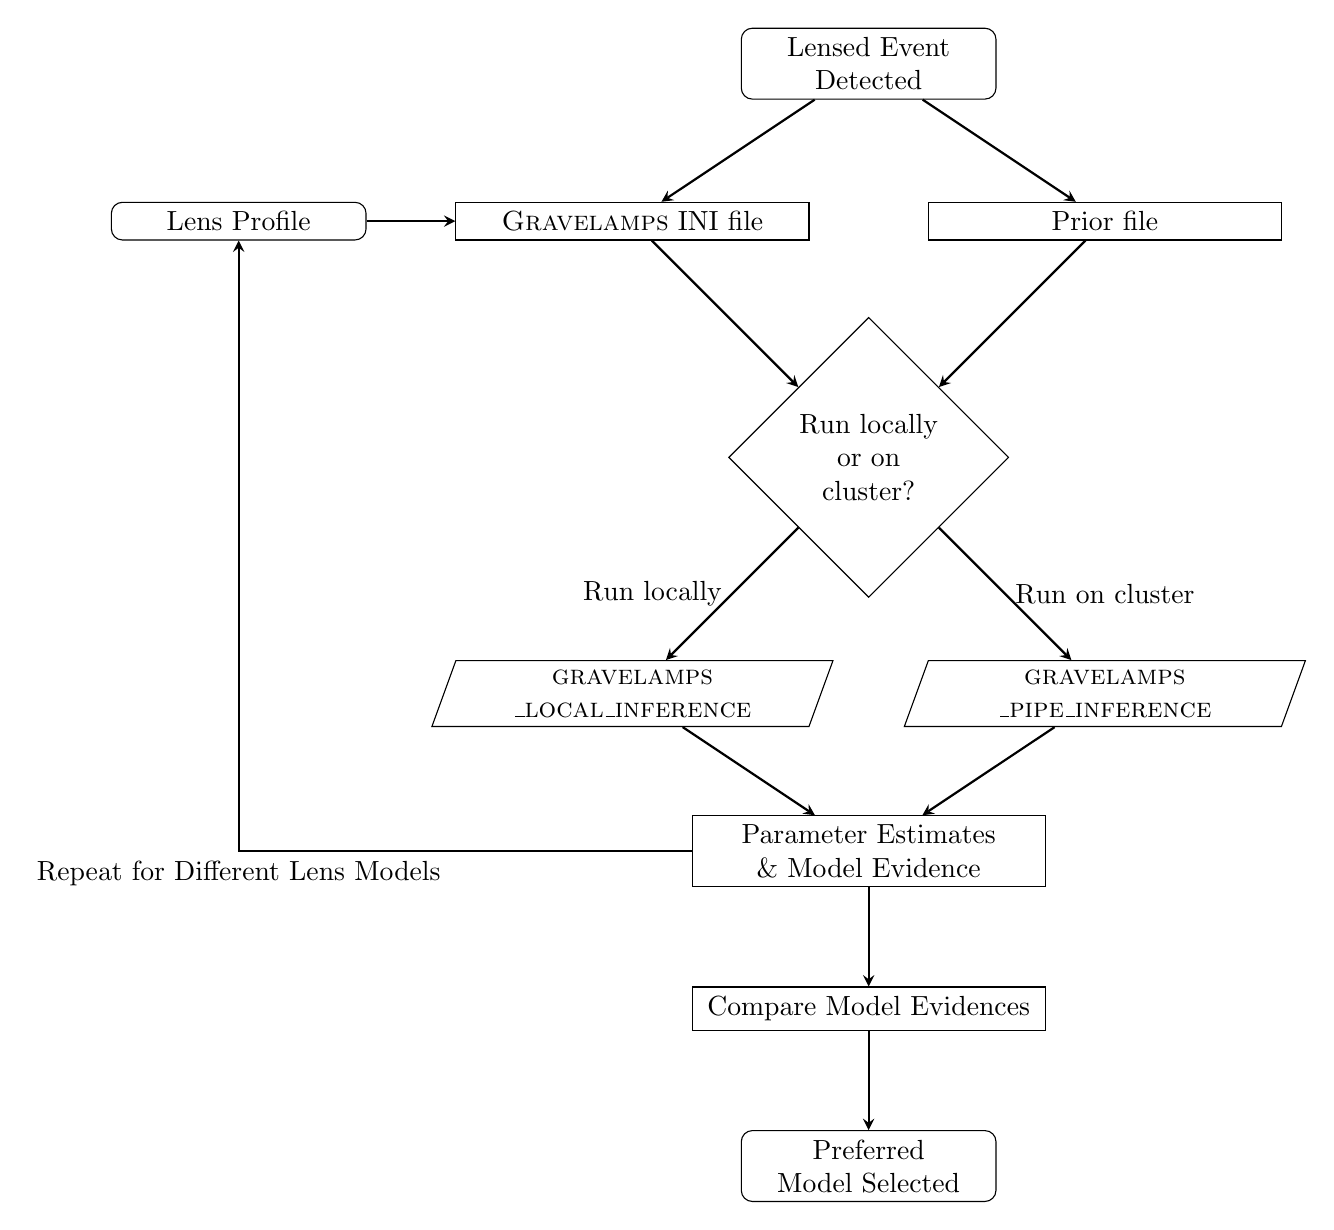
\begin{tikzpicture}[node distance=2cm]
	\node (event) [startstop] {Lensed Event Detected};

	\node (ini) [process, below of=event, xshift=-3cm] {\textsc{Gravelamps} INI file};
	\node (prior) [process, below of=event, xshift=3cm] {Prior file};
	\node (modchoice) [startstop, left of=ini, xshift=-3cm] {Lens Profile}; 

	\node (clusloc) [decision, below of=ini, xshift=3cm, yshift=-1cm] {Run locally or on cluster?};

	\draw [arrow] (modchoice) -- (ini);
	\draw [arrow] (event) -- (ini);
	\draw [arrow] (event) -- (prior);
	\draw [arrow] (ini) -- (clusloc);
	\draw [arrow] (prior) -- (clusloc);

	\node (localrun) [io, below of=clusloc, xshift=-3cm, yshift=-1cm] {\textsc{gravelamps\\\_local\_inference}};
	\node (clusterrun) [io, below of=clusloc, xshift=3cm, yshift=-1cm] {\textsc{gravelamps\\\_pipe\_inference}};

	\draw [arrow] (clusloc) -- node[anchor=east] {Run locally} (localrun);
	\draw [arrow] (clusloc) -- node[anchor=west] {Run on cluster} (clusterrun);

	\node (modev) [process, below of=localrun, xshift=3cm] {Parameter Estimates \& Model Evidence};

	\draw [arrow] (localrun) -- (modev);
	\draw [arrow] (clusterrun) -- (modev);
	\draw [arrow] (modev) -| node[anchor=north] {Repeat for Different Lens Models} (modchoice); 

	\node (evcomp) [process, below of=modev] {Compare Model Evidences}; 

	\node (bayes) [startstop, below of=evcomp] {Preferred Model Selected};

	\draw [arrow] (modev) -- (evcomp);
	\draw [arrow] (evcomp) -- (bayes); 
\end{tikzpicture}

\section*{Inference Flowchart}
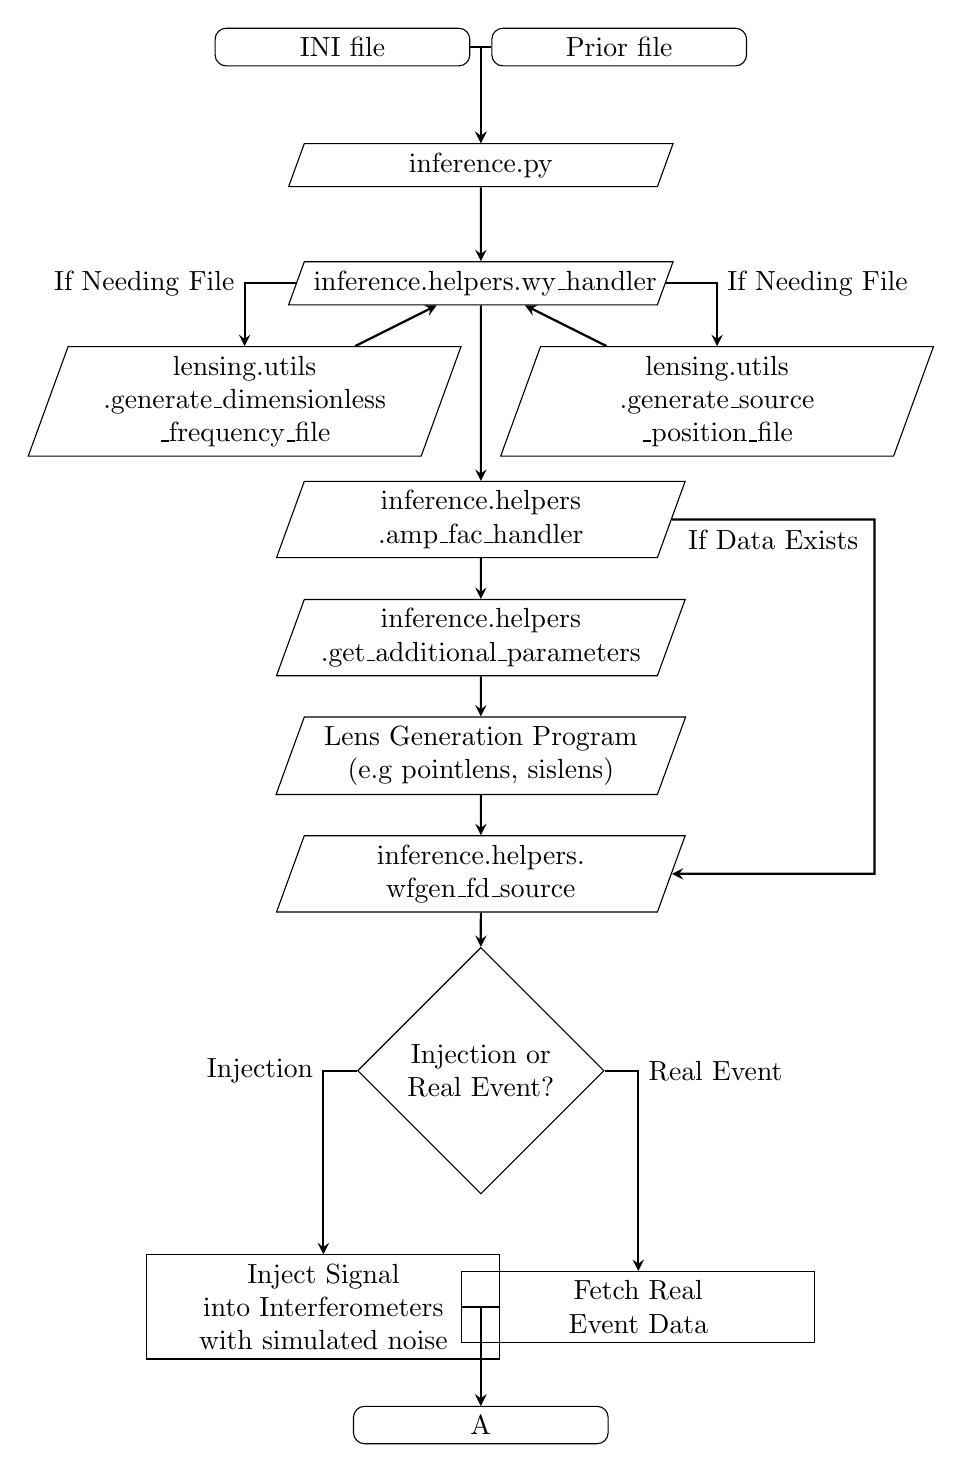
\begin{tikzpicture}[node distance=1.5cm]
	\node (ini) [startstop, xshift=-50] {INI file}; 
	\node (prior) [startstop, xshift=50] {Prior file}; 

	\node (inference) [io, below of=ini, xshift=50] {inference.py};

	\draw [arrow] (ini) -| (inference);
	\draw [arrow] (prior) -| (inference);

	\node (wyhandler) [io, below of=inference] {inference.helpers.wy\_handler};

	\draw [arrow] (inference) -- (wyhandler); 

	\node (gendimfreq) [io, below of=wyhandler, xshift=-3cm] {lensing.utils\\.generate\_dimensionless\\\_frequency\_file};
	\node (gensourpos) [io, below of=wyhandler, xshift=3cm] {lensing.utils\\.generate\_source\\\_position\_file};

	\node (ampfachandler) [io, below of=gendimfreq, xshift=3cm] {inference.helpers\\.amp\_fac\_handler};

	\draw [arrow] (wyhandler) -| node[anchor=east] {If Needing File} (gendimfreq);
	\draw [arrow] (wyhandler) -| node[anchor=west] {If Needing File} (gensourpos); 

	\draw [arrow] (gendimfreq) -- (wyhandler);
	\draw [arrow] (gensourpos) -- (wyhandler);
	\draw [arrow] (wyhandler) -- (ampfachandler);

	\node (addpar) [io, below of=ampfachandler] {inference.helpers\\.get\_additional\_parameters};

	\draw [arrow] (ampfachandler) -- (addpar);

	\node (lensgen) [io, below of=addpar] {Lens Generation Program \\ (e.g pointlens, sislens)};

	\draw [arrow] (addpar) -- (lensgen);

	\node (wfgenfdsource) [io, below of=lensgen] {inference.helpers.\\wfgen\_fd\_source};

	\draw [arrow] (lensgen) -- (wfgenfdsource);
	\draw [arrow] (ampfachandler) -- node[anchor=north] {If Data Exists} ++ (5cm, 0) |- (wfgenfdsource);

	\node (inject) [decision, below of=wfgenfdsource, yshift=-1cm] {Injection or Real Event?};

	\node (injection) [process, below of=inject, yshift=-1.5cm, xshift=-2cm] {Inject Signal\\ into Interferometers\\ with simulated noise};
	\node (realevent) [process, below of=inject, yshift=-1.5cm, xshift=2cm] {Fetch Real \\ Event Data};

	\draw [arrow] (wfgenfdsource) -- (inject);
	\draw [arrow] (inject) -| node[anchor=0] {Injection} (injection);
	\draw [arrow] (inject) -| node[anchor=west] {Real Event} (realevent);
	\node (breaker) [startstop, below of=injection, xshift=2cm] {A};

	\draw [arrow] (injection) -| (breaker);
	\draw [arrow] (realevent) -| (breaker); 
\end{tikzpicture} 

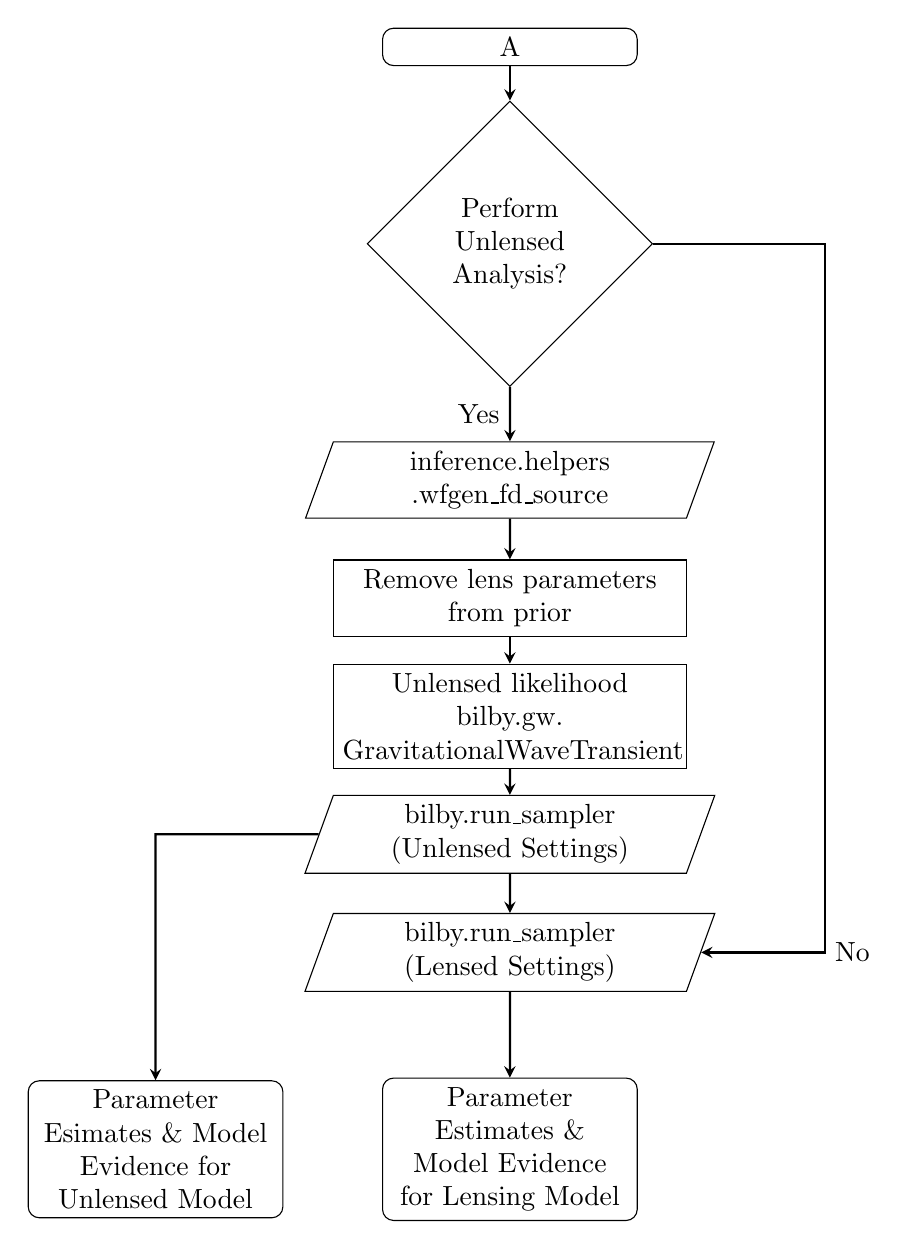
\begin{tikzpicture}[node distance=1.5cm]
	\node (breaker) [startstop] {A};
	\node (unlenseddecision) [decision, below of=breaker, yshift=-1cm] {Perform Unlensed Analysis?};
	\node (wfgenfdsource) [io, below of=unlenseddecision, yshift=-1.5cm] {inference.helpers\\.wfgen\_fd\_source}; 

	\draw [arrow] (breaker) -- (unlenseddecision);
	\draw [arrow] (unlenseddecision) -- node[anchor=east] {Yes} (wfgenfdsource);

	\node (unlensedpriors) [process, below of=wfgenfdsource] {Remove lens parameters\\ from prior};
	\node (unlensedlikelihood) [process, below of=unlensedpriors] {Unlensed likelihood \\ bilby.gw.\\GravitationalWaveTransient}; 

	\draw[arrow] (wfgenfdsource) -- (unlensedpriors);
	\draw[arrow] (unlensedpriors) -- (unlensedlikelihood); 

	\node (unlensedrun) [io, below of=unlensedlikelihood] {bilby.run\_sampler \\ (Unlensed Settings)};

	\draw [arrow] (unlensedlikelihood) -- (unlensedrun); 

	\node (lensedrun) [io, below of=unlensedrun] {bilby.run\_sampler \\ (Lensed Settings)};

	\draw [arrow] (unlensedrun) -- (lensedrun);
	\draw [arrow] (unlenseddecision) -- ++ (4cm, 0) |- node[anchor=west] {No} (lensedrun);

	\node (end) [startstop, below of=lensedrun, yshift=-1cm] {Parameter Estimates \& Model Evidence for Lensing Model};
	\node (endun) [startstop, left of=end, xshift=-3cm] {Parameter Esimates \& Model Evidence for Unlensed Model};

	\draw[arrow] (lensedrun) -- (end);
	\draw[arrow] (unlensedrun) -- ++ (-4cm, 0) -| (endun);
\end{tikzpicture}

\end{document}
